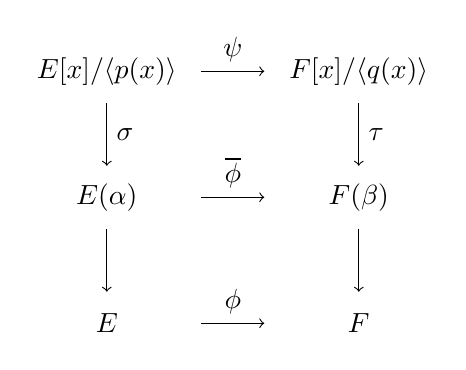
\begin{tikzpicture}[scale=0.8]

\draw [<-] (0,0.5) -- (0,1.5);
\draw [<-] (0,2.5) -- (0,3.5);


\draw [<-] (4,0.5) -- (4,1.5);
\draw  [<-] (4,2.5) -- (4,3.5);


\draw [->] (1.5,0) -- (2.5,0);
\draw [->] (1.5,2) -- (2.5,2);
\draw [->] (1.5,4) -- (2.5,4);


\node at (0,0)  {$E$};
\node at (4,0)  {$F$};

\node at (0,2)  {$E(\alpha)$};
\node at (4,2)  {$F(\beta)$};

\node at (0,4)  {$E[x] / \langle p(x) \rangle$};
\node at (4,4)  {$F[x]/\langle q(x) \rangle$};

\node [above] at (2,0) {$\phi$};
\node [above] at (2,2) {$\overline{\phi}$};
\node [above] at (2,4) {$\psi$};

\node [right] at (0,3) {$\sigma$};
\node [right] at (4,3) {$\tau$};

\end{tikzpicture}
